\documentclass{article}
\usepackage[paperwidth=160mm,paperheight=128mm,margin=6mm]{geometry}
\usepackage{tikz}
\pagestyle{empty}
\setlength{\parindent}{0pt}
\usetikzlibrary{arrows.meta,positioning}

\renewcommand{\familydefault}{\sfdefault}
\begin{document}
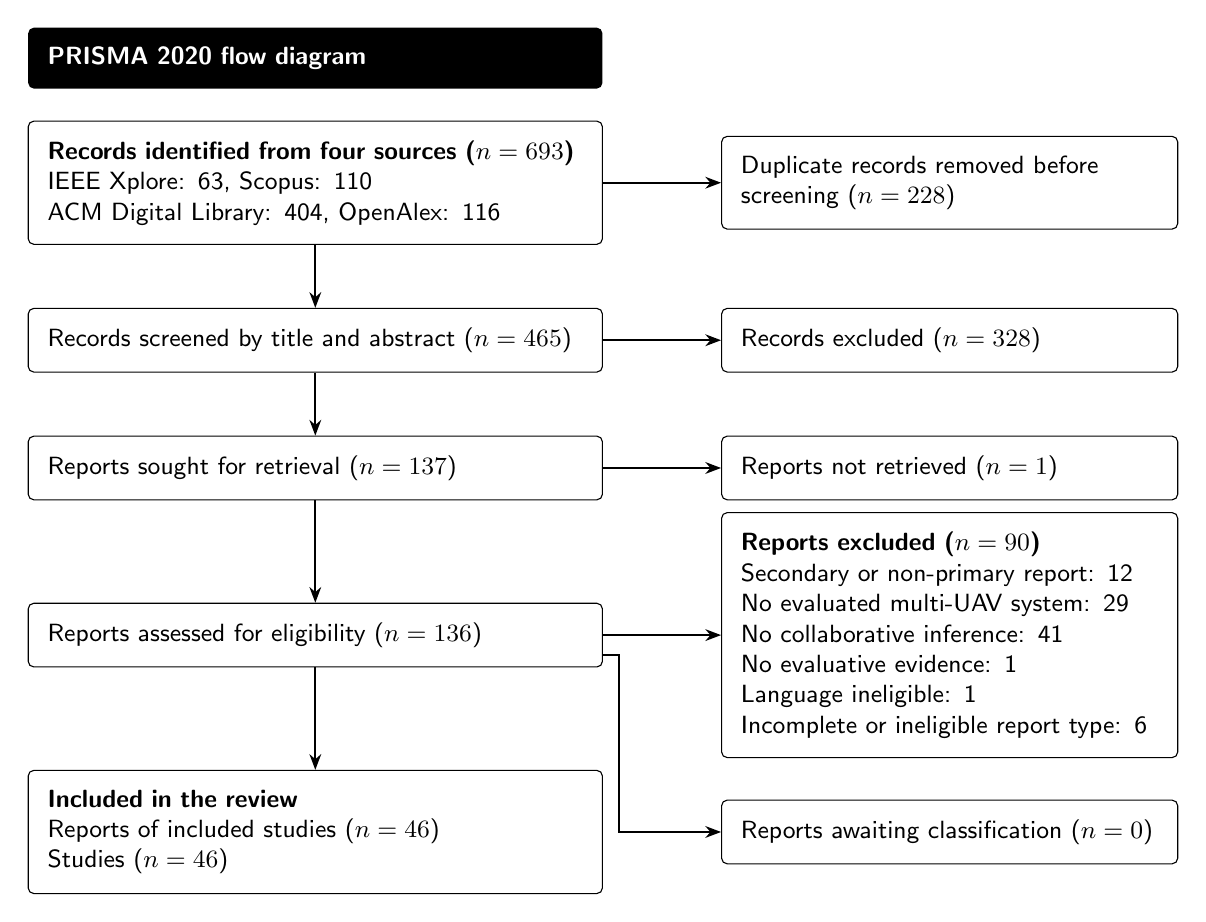
\begin{tikzpicture}[
  main/.style={draw, rounded corners=2pt, text width=68mm, inner sep=7pt, align=left, font=\small},
  detail/.style={main,text width=53mm},
  stage/.style={main,draw=none,fill=black,text=white,text width=68mm},
  fork/.style={-{Stealth[length=2mm]},line width=.6pt},
  node distance=8mm and 15mm,
]
\node[stage] (header) {\textbf{PRISMA 2020 flow diagram}};
\node[main,below=4mm of header] (raw) {\textbf{Records identified from four sources ($n=693$)}\\
IEEE Xplore: 63, Scopus: 110\\ ACM Digital Library: 404, OpenAlex: 116};
\node[detail,right=of raw] (dup) {Duplicate records removed before screening ($n=228$)};
\node[main,below=of raw] (screen) {Records screened by title and abstract ($n=465$)};
\node[detail,right=of screen] (screenex) {Records excluded ($n=328$)};
\node[main,below=of screen] (sought) {Reports sought for retrieval ($n=137$)};
\node[detail,right=of sought] (missing) {Reports not retrieved ($n=1$)};
\node[main,below=13mm of sought] (assessed) {Reports assessed for eligibility ($n=136$)};
\node[detail,right=of assessed] (fulltextex) {\textbf{Reports excluded ($n=90$)}\\
Secondary or non-primary report: 12\\ No evaluated multi-UAV system: 29\\ No collaborative inference: 41\\ No evaluative evidence: 1\\ Language ineligible: 1\\ Incomplete or ineligible report type: 6};
\node[main,below=13mm of assessed] (included) {\textbf{Included in the review}\\
Reports of included studies ($n=46$)\\ Studies ($n=46$)};
\node[detail,right=of included] (pending) {Reports awaiting classification ($n=0$)};
\foreach \from/\to in {raw/screen,screen/sought,sought/assessed,assessed/included,raw/dup,screen/screenex,sought/missing,assessed/fulltextex}
  \draw[fork] (\from) -- (\to);
\draw[fork] ([yshift=-2.5mm]assessed.east) -- ++(2mm,0) |- (pending.west);
\end{tikzpicture}
\end{document}
